Figures:

\begin{figure}[htbp]
	\centering\small
	\begin{tabular}{cc}
		\fbox{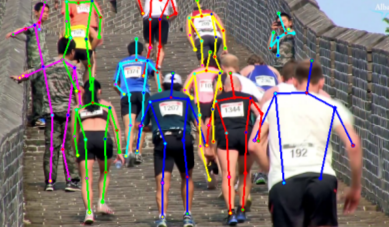
\includegraphics[width=0.43\textwidth]{poseEstimation}} &		% JPEG file
		\fbox{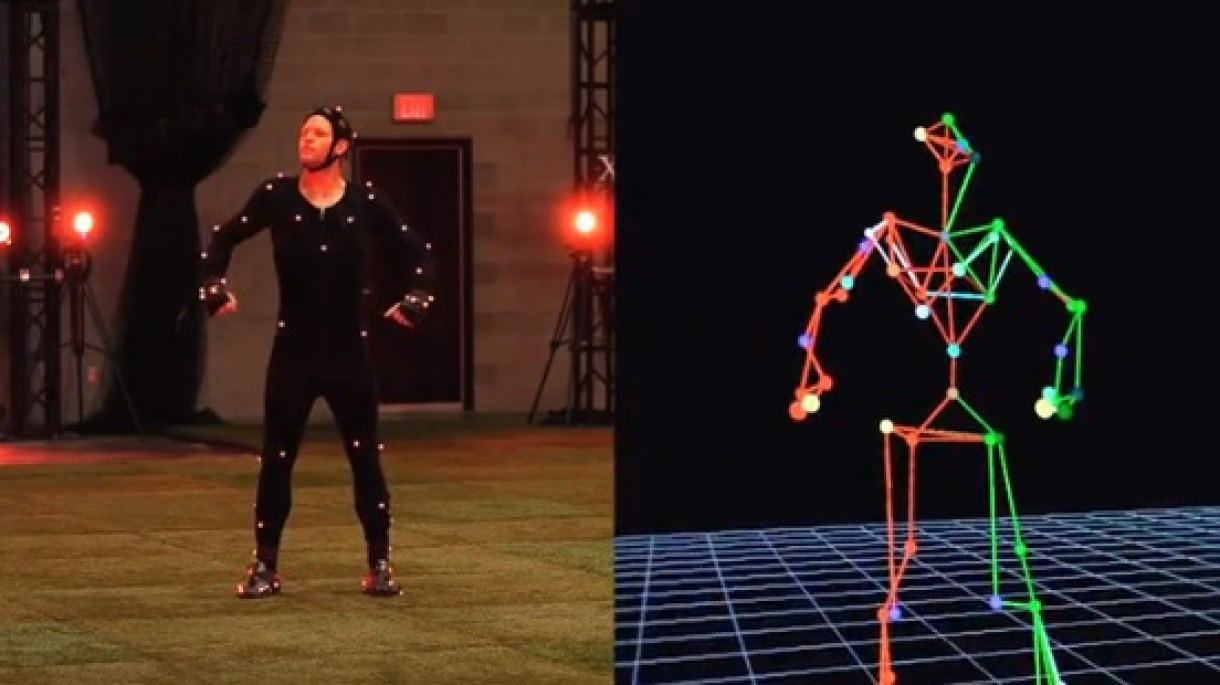
\includegraphics[width=0.45\textwidth]{motionCapture}} 
		\\	% PNG file
		(a) & (b) 
	\end{tabular}
	\caption{Multi-person pose estimation~(a) \cite{poseEstimation} and optical Motion Capture with markers~(b) \cite{MotionCapture}.} 
	\label{fig:motivation}
\end{figure}

\begin{figure}[H]
	\centering\small
	\begin{tabular}{cc}
		\fbox{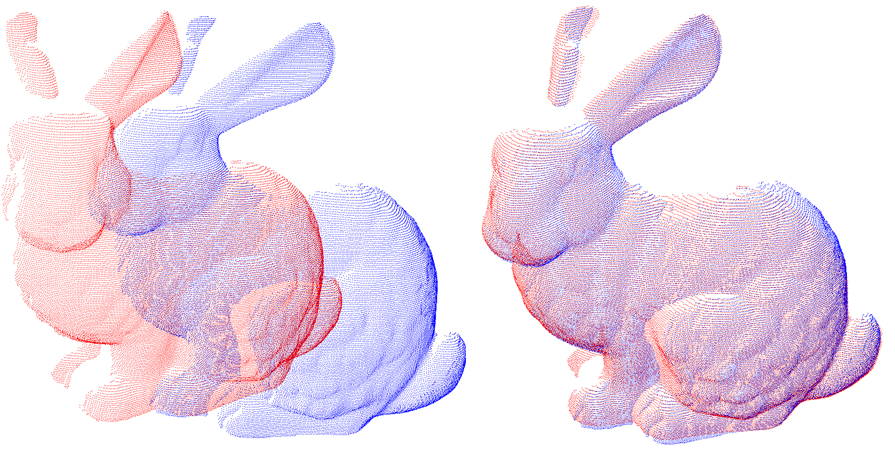
\includegraphics[width=0.43\textwidth]{stanfordBunny}} &		% JPEG file
		\fbox{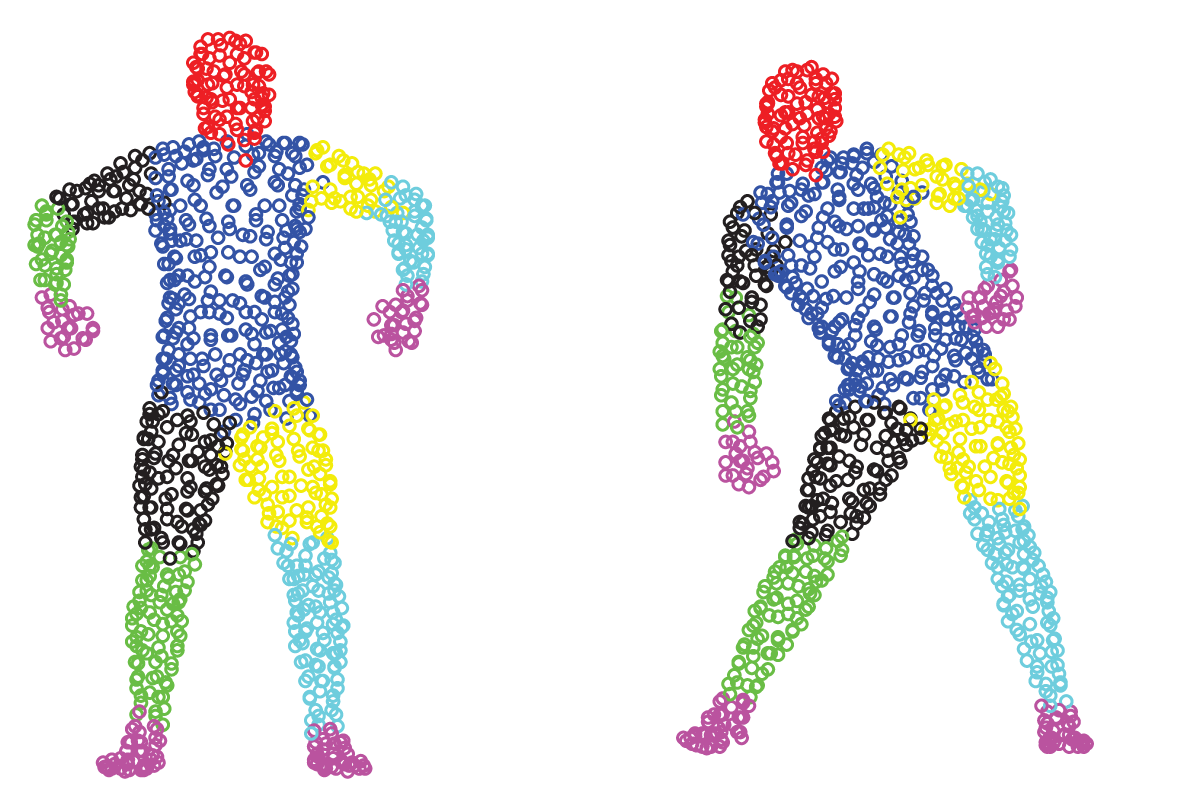
\includegraphics[width=0.45\textwidth]{nonrigidregistration}} 
		\\	% PNG file
		(a) & (b) 
	\end{tabular}
	\caption{Rigid registration of the stanford bunny~(a) \cite{stanfordBunny} and non-rigid registration of a human~(b) \cite{registrationHuman} by detecting its rigid parts.}
	
	\label{fig:registration}
\end{figure}\textbf{}

\begin{figure}
	\centering
	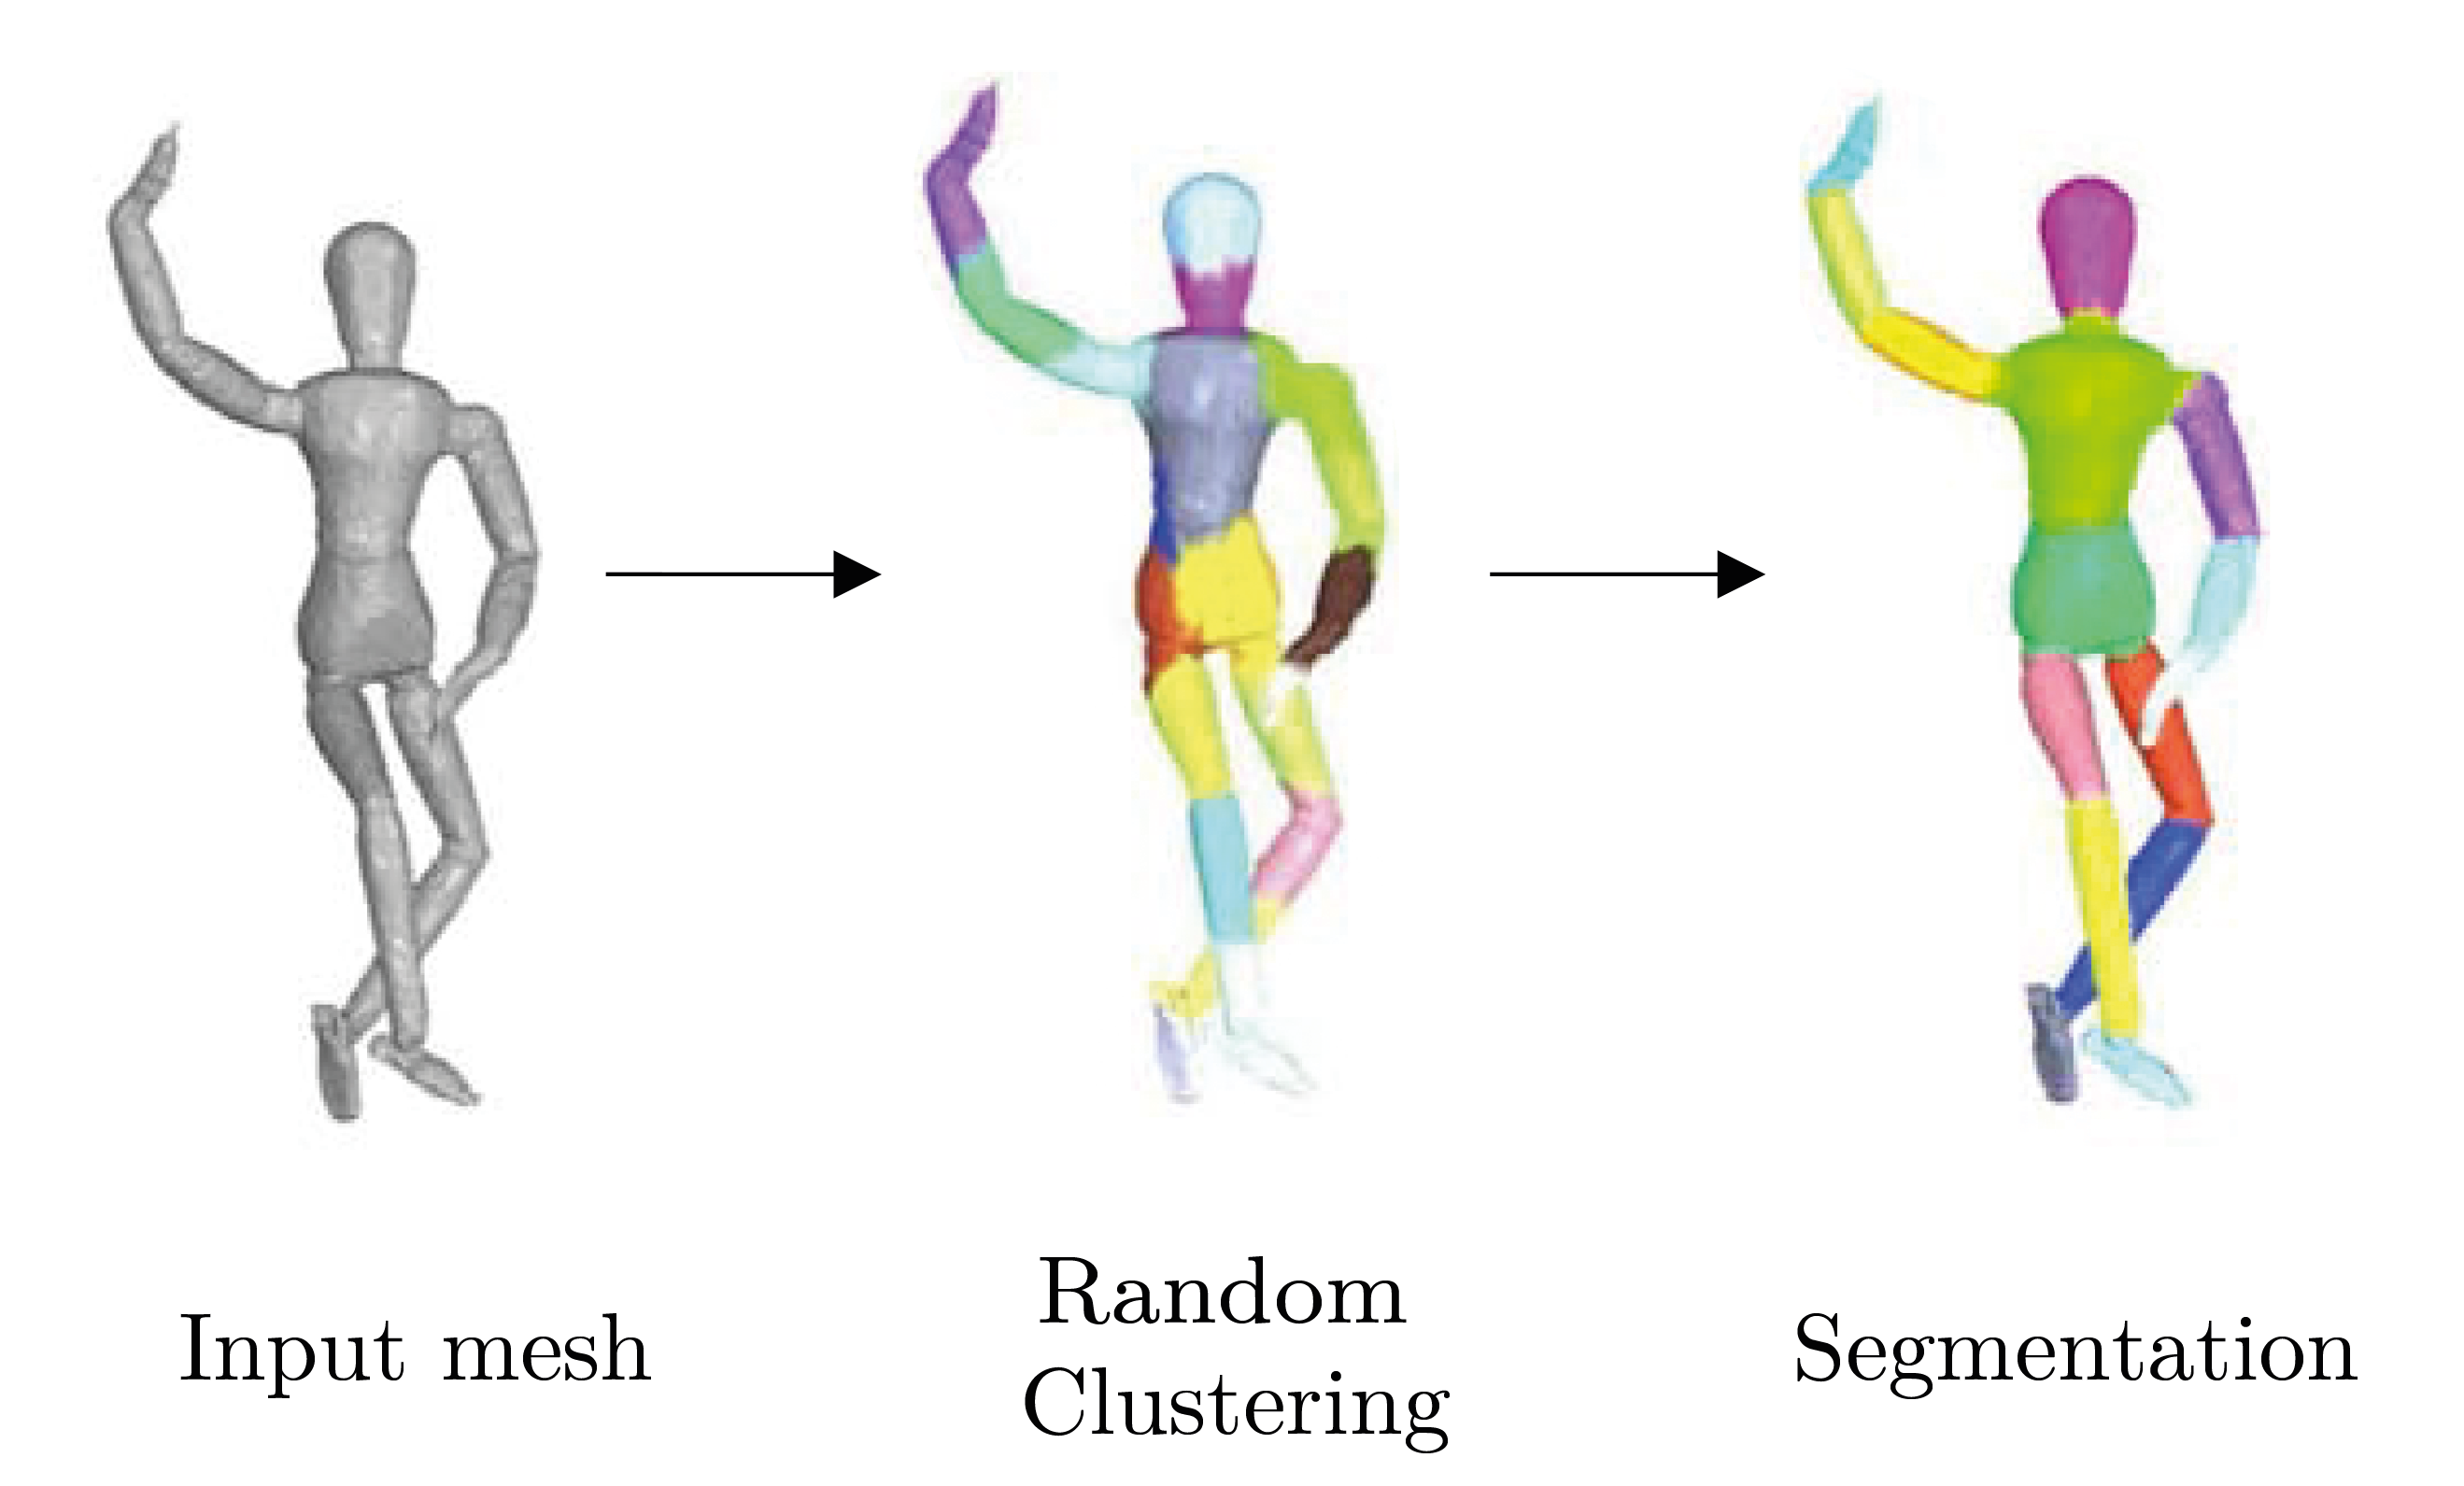
\includegraphics[width=0.7\linewidth]{anguelov}
	\caption{Segmentation a template mesh $M$ into its rigid parts by applying random clustering and a probabilistic framework to iteratively detect associating parts in another mesh \cite{Anguelov04}.}
	\label{fig:correlatedcorrespondance}
\end{figure}

\begin{figure}[H]
	\centering\small
	\begin{tabular}{cc}
		\fbox{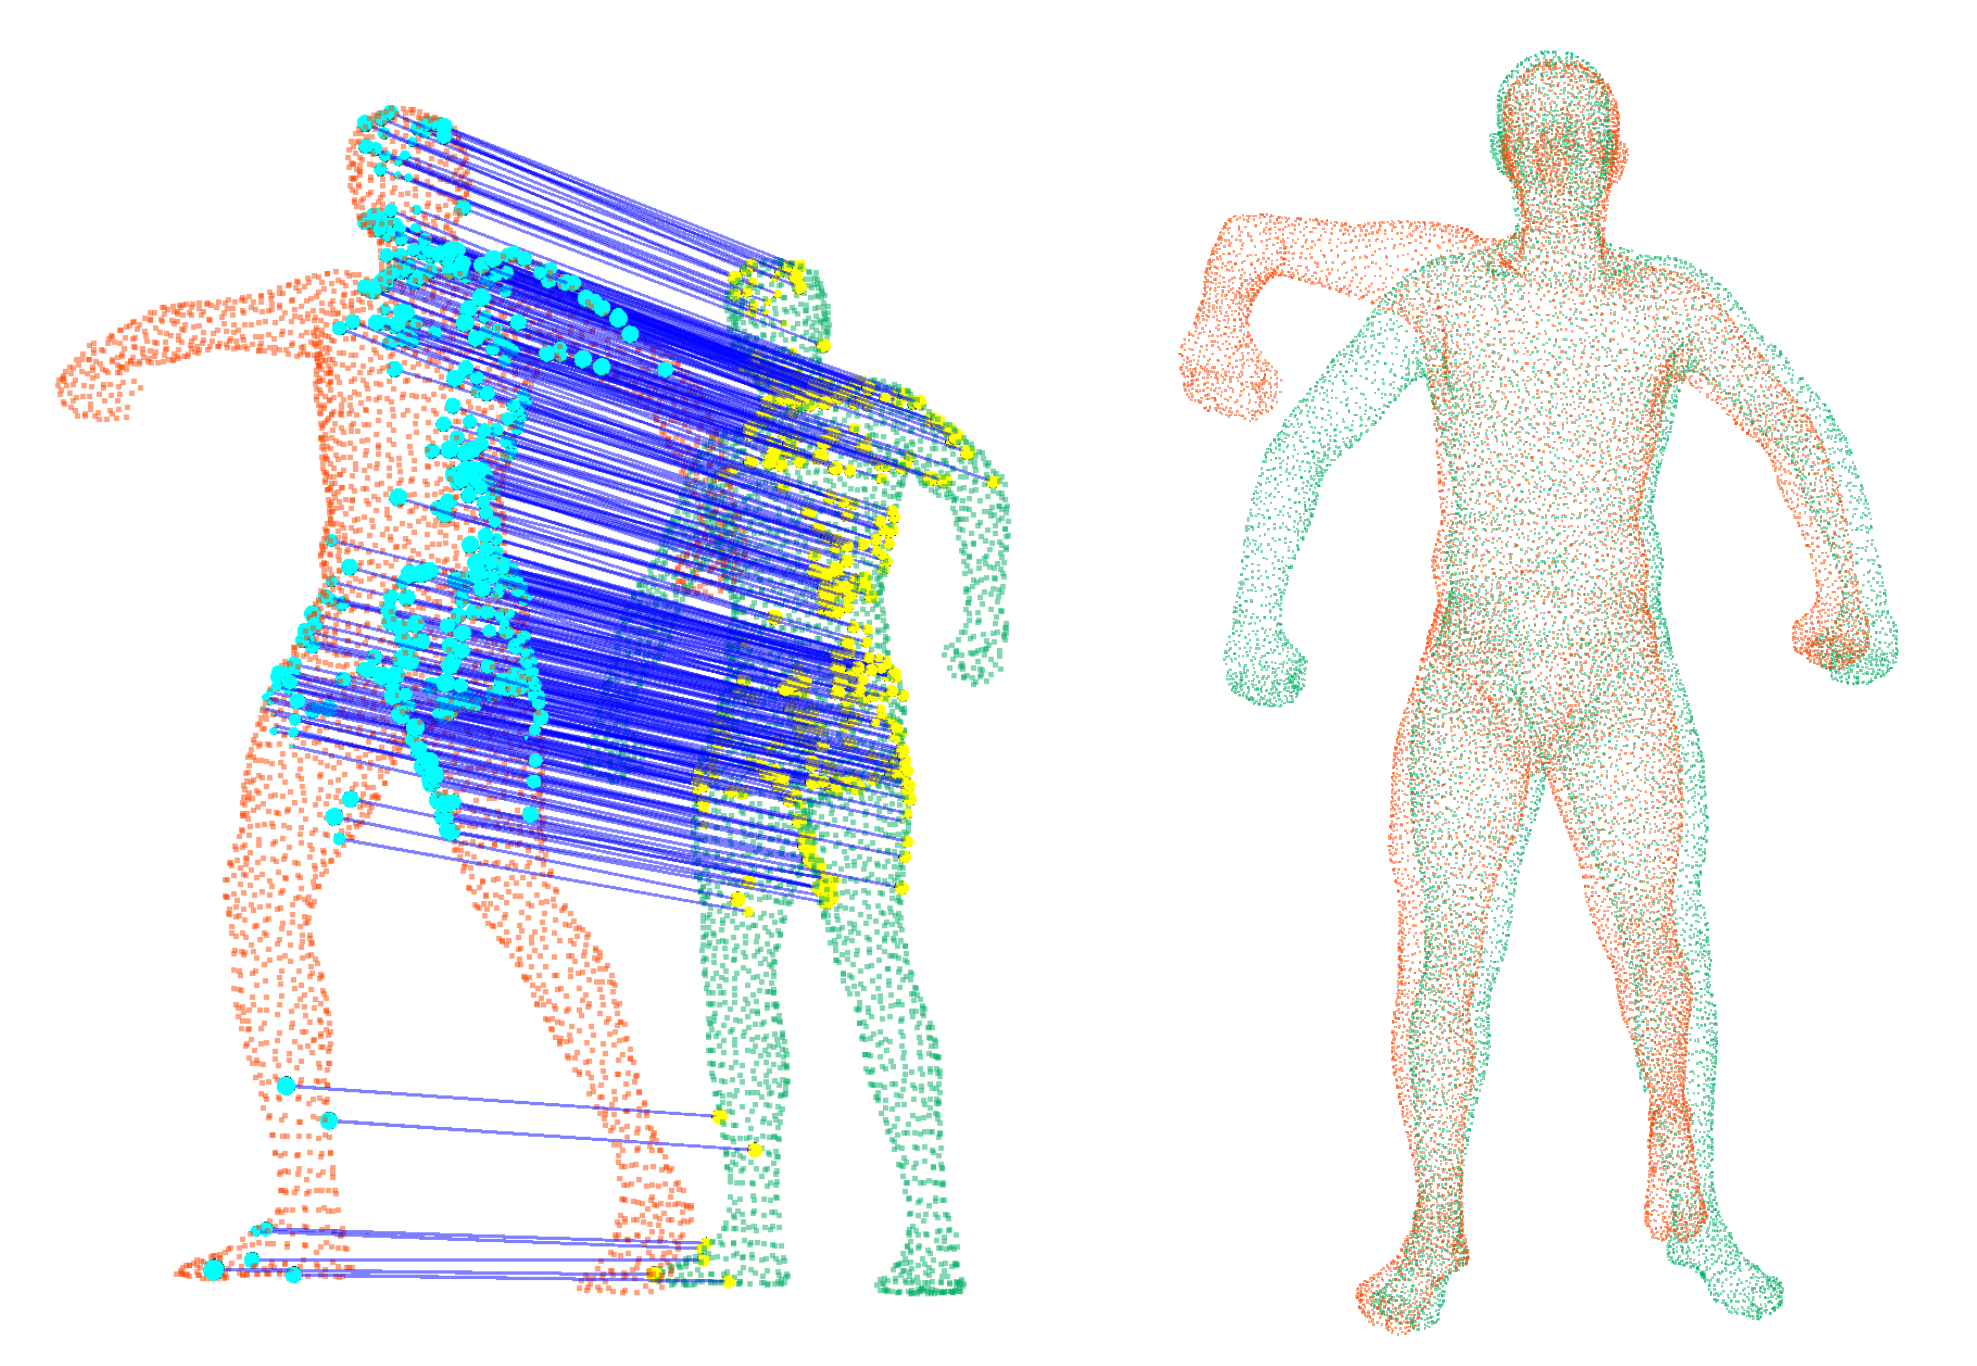
\includegraphics[width=0.45\textwidth]{LRP_body}} &	
		\fbox{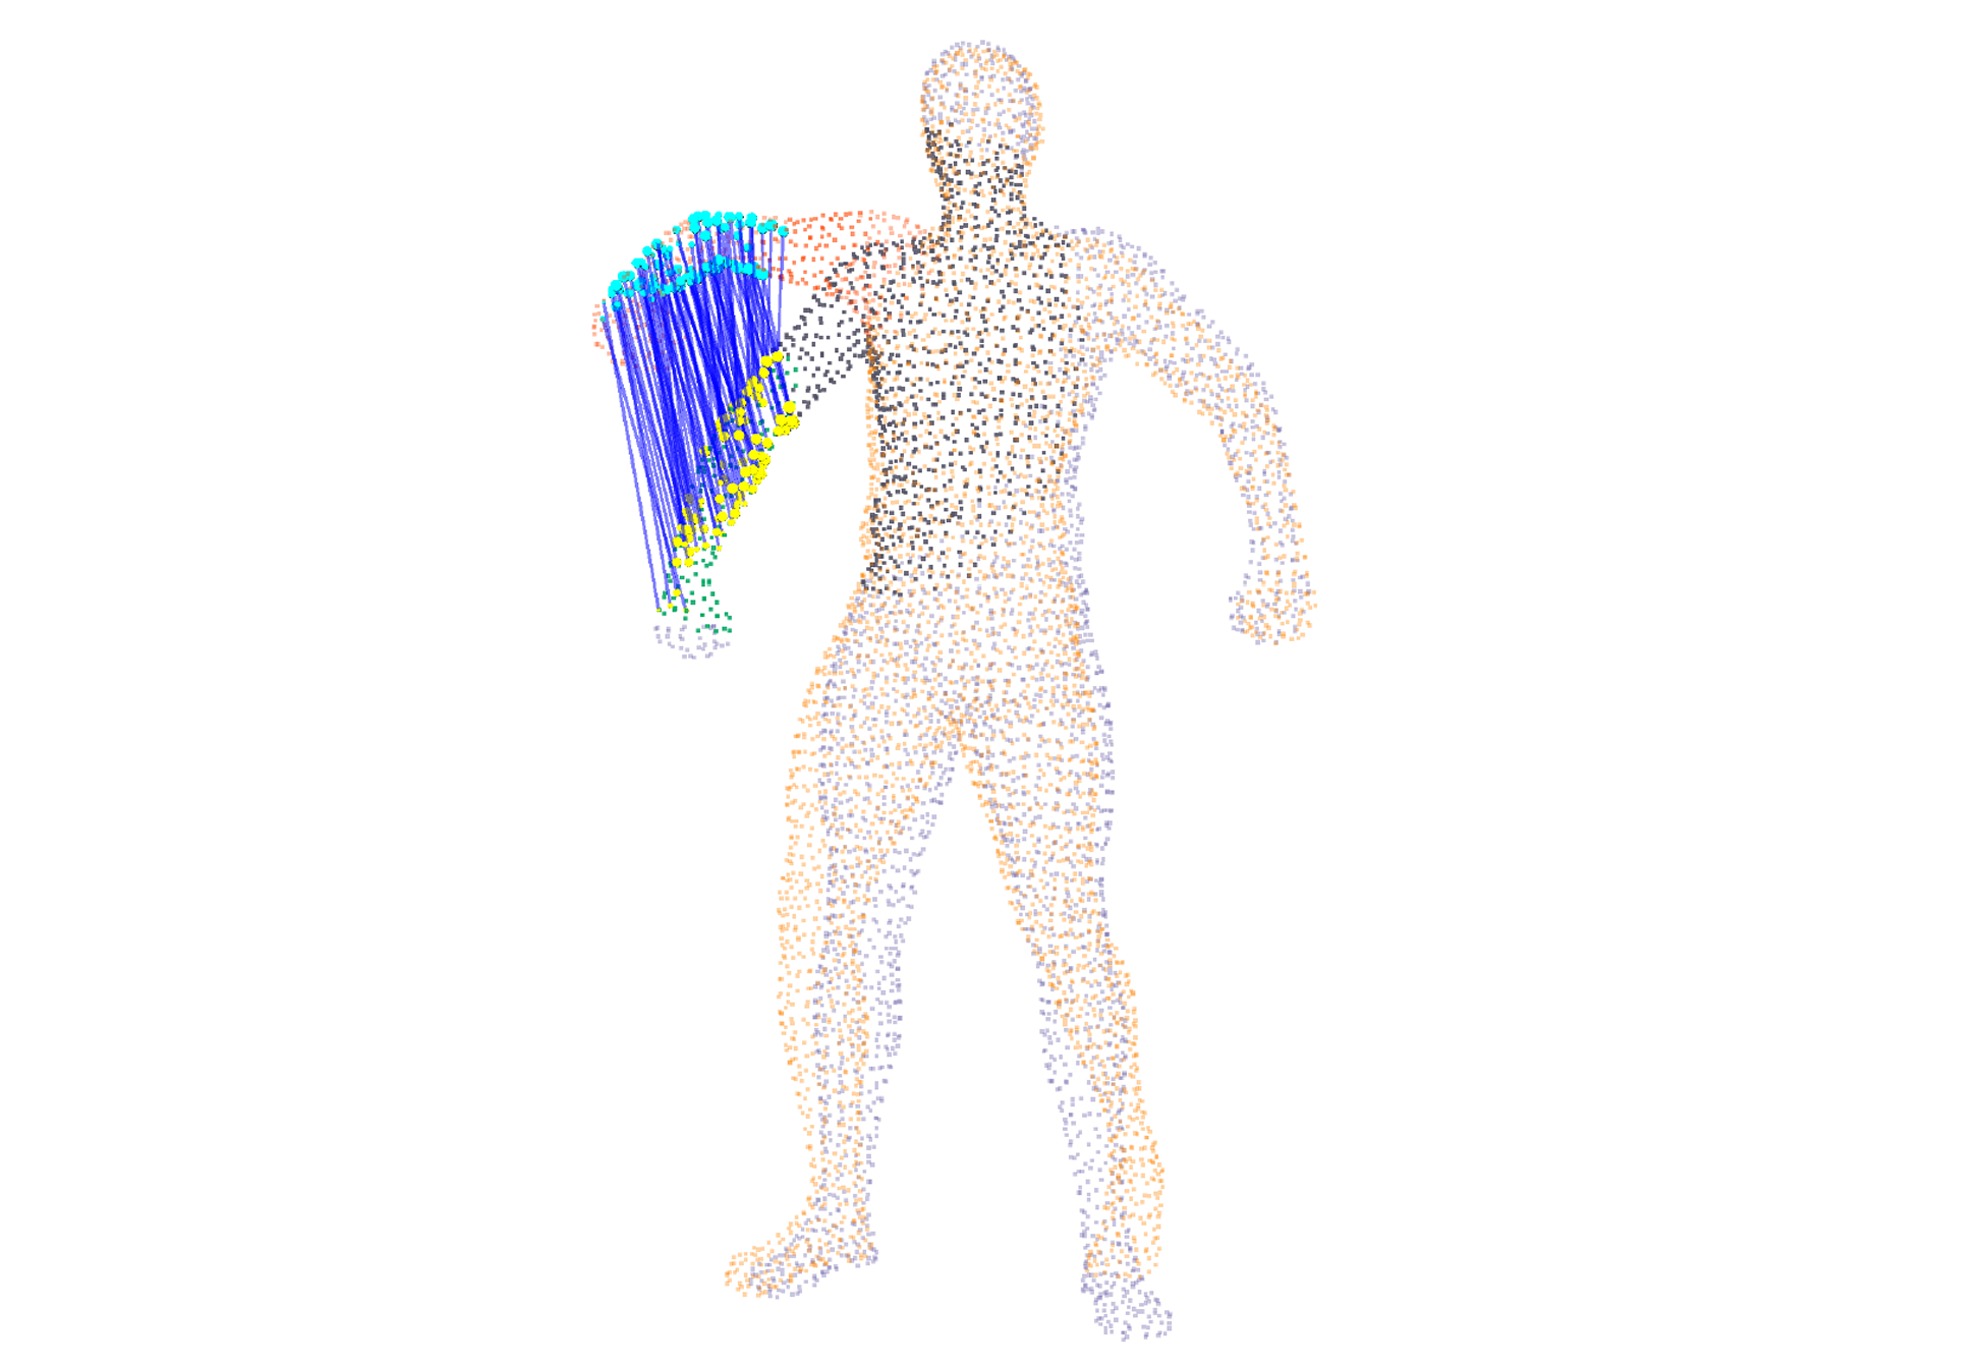
\includegraphics[width=0.45\textwidth]{LRP_arm}} 
		\\
		(a) & (b) 
	\end{tabular}
	\caption{Detecting the largest rigid part of an object~(a), and align the object to recursively detect linking parts to the LRP~(b) \cite{guo2016correspondence}.} 
	\label{fig:LRP_algorithm}
\end{figure}

\begin{figure}[H]
	\centering\small
	\begin{tabular}{cc}
		\fbox{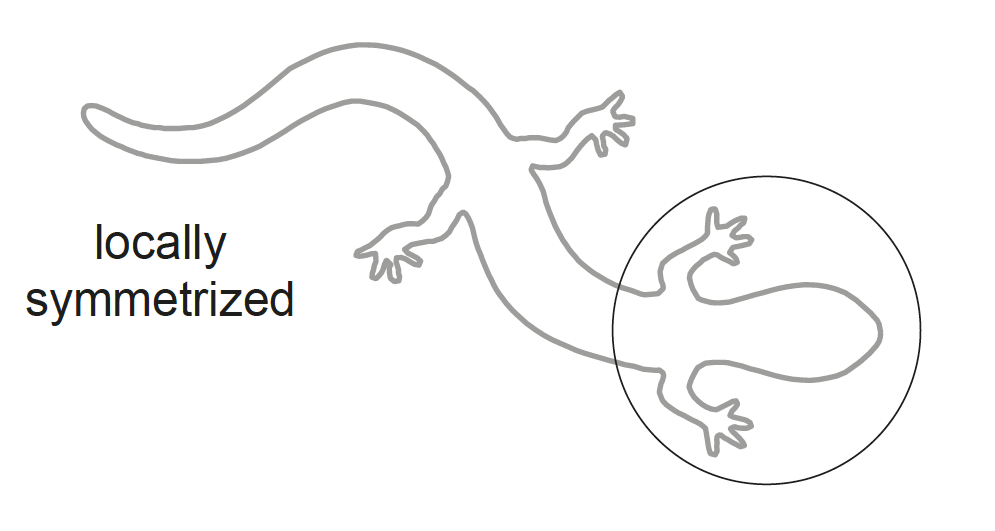
\includegraphics[width=0.45\textwidth]{Symmetrization1}} &
		\fbox{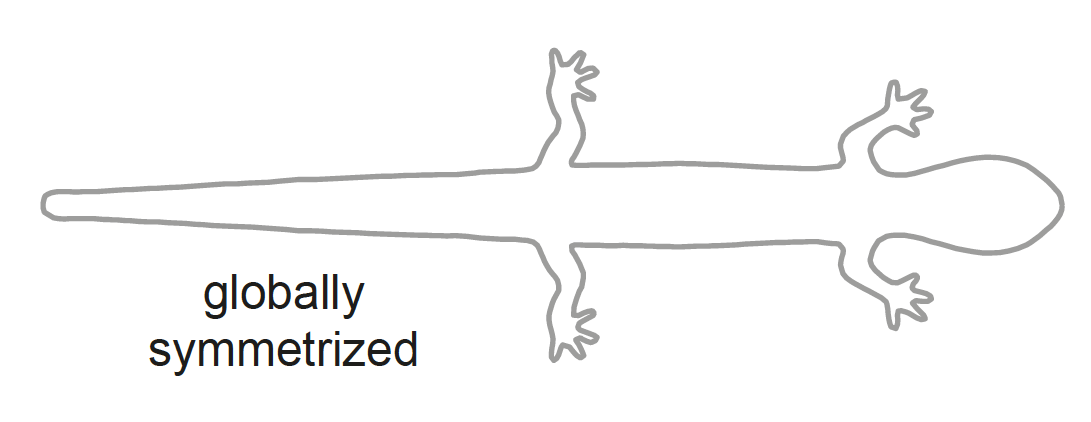
\includegraphics[width=0.45\textwidth]{Symmetrization2}} 
		\\
		(a) & (b) 
	\end{tabular}
	\caption{Detection of the rigid parts of an object by local~(a) and global~(b) Symmetrization \cite{Mitra07}.} 
	\label{fig:Symmetrization}
\end{figure}